
\documentclass[a4paper]{article}
\usepackage[utf8]{inputenc}
\usepackage[T1]{fontenc}
\usepackage{amsmath, amssymb}
\usepackage{xspace}
\usepackage[frenchb]{babel}
\usepackage{hyperref}
\usepackage{graphicx}
\usepackage{caption}
\usepackage{subcaption}

\title{Génération de codes d'inférences probabilistes	}
\author{Marvin Lavechin et Pierre Stefani}

\begin{document}
\maketitle
\thispagestyle{empty}

\newpage
\thispagestyle{empty}
\pagenumbering{Alph}
\setcounter{page}{0}
~
\newpage
\tableofcontents

\newpage
 \section{Présentation du projet}
 De Mars à Juillet 2014, encadré par Mr Pierre Henri Wuillemin, chercheur à l'Université Pierre et Marie Curie, nous avons 
 travaillé sur la génération d'un code pour calculer des probabilités d'un réseau bayésien.
 \par \medbreak
 Les réseaux bayésiens sont des faisceaux de probabilités, ordonnés par des liens de parentés. Chacun des événements du réseau bayésien
 possède une table de probabilités dépendant des valeurs prises par ses parents. L'information peut ainsi être diffusé dans de tels réseaux.
 Le projet metaGenBayes utilise cette diffusion, appelé inférence, pour calculer une probabilité spécifique appelé target à partir d'un 
 évènement certain(hard evidence) ou connu(soft evidence). Nous reviendrons sur ce vocabulaire plus en détail par la suite.
 Dans un cadre classique, ce calcul de probabilités selon des observations : $P(X|e)$ est simple. Toutefois, les modèles étant très vite complexes, l'inférence probabiliste devient
 un problème NP-difficile.
 \begin{figure}[h!]
  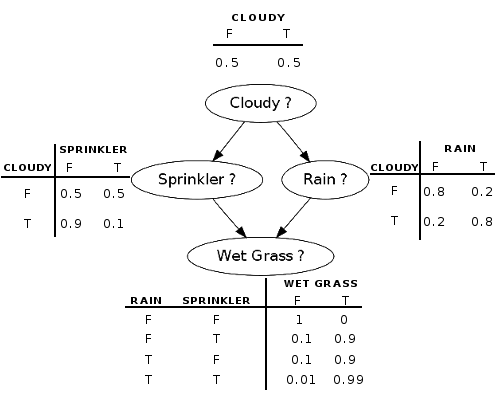
\includegraphics[width=\linewidth]{Images/Waterprinkler.png}
  \caption{Exemple de réseau bayésien}
  \label{fig:bn1}
 \end{figure}
\par \medbreak
Le but du projet était de créer un moteur d'inférence probabiliste, qui n'allait pas faire le calcul mais générer des codes calculatoires dans différents langages cibles. Ce moteur
s'appuie sur certaines bibliothèques lip6, comme par exemple pyAgrum.

\newpage
 \section{Présentation du problème}
  \subsection{Calcul de probabilité}
   \subsubsection{Quelques formules}
   
Comme explicité dans la courte présentation, l'inférence probabiliste s'appuie sur des probabilités conditionnelles, régies par quelques lois de calcul qu'il est important d'introduire:\\
Soient A et B deux événements quelconques d'un même univers. On s'intéresse à ce que devient la probabilité de A lorsqu'on apprend que B est déjà réalisé. On note $P(A|B)$ et on lit "probabilité de A sachant B".
La définition mathématique de $P(A|B)$ est :
$$P(A|B) = \frac{P(A\cap B)}{P(B)} = \frac{P(B|A)P(A)}{P(B)} ,\quad P(B)\ne 0$$
\hfill(Formule de Bayes)
\newline
~
\newline
Cette formule s'écrit aussi :
$P(A|B) \quad \alpha \quad P(A) \times P(B|A)$\footnote{$P(A|B)$ est la loi à posteriori, $P(A)$ la loi à priori et $P(B|A)$ la vraisemblance, tandis que P(B) sert de coefficient normalisateur}
\newline
Ceci nous amène à considérer deux autres formules.
Soit $(A_i)_{i\in I}$ un système complet d'événements de probabilités non nulles. Alors pour tout événement $B$ on a : 
$$P(B)=\sum_{i\in I} P(A_i\cap B)=\sum_{i\in I} P(A_i)P(B|A_i)$$
\hfill(Formule des probabilités totales)
\newline
~
\newline
Si $P(A_1 \cap \ldots \cap A_n) \ne 0$, on a :
$$P(A_1 \cap \ldots \cap A_n) = \prod_{i = 1}^{n} P(A_i|A_{i+1} \cap \ldots \cap A_n)$$
\hfill(Formule des probabilités composées)

    \subsubsection{Calcul au sein d'une table de probabilité jointe}
Soient $A_1,A_2,A_3$ trois variables aléatoires binaires. On peut écrire une table listant toutes les combinaisons possibles de ces 3 variables, qui sont au nombre de $2^3$.\newline
En effet, on a :
\begin{align*}
\begin{pmatrix} A_1 = true & A_2 = true & A_3 = true\end{pmatrix}\\
\begin{pmatrix} A_1 = false & A_2 = true & A_ 3 = true\end{pmatrix} \\
\begin{pmatrix} A_1 = true & A_2 = false & A_ 3 = true\end{pmatrix} \\ etc...
\end{align*}
Pour chacune des combinaisons, supposons que nous disposions de la probabilité jointe de cette combinaison.\newline
Si l'on veut la probabilité $P(A_1 \cap A_2)$, la formule des probabilités totales nous dit qu'il suffit qu'on somme les probabilités des combinaisons de la table pour laquelle $A_1$ est vrai et $A_2$ l'est aussi.
\newline
Si l'on veut la probabilité $P(A_1|A_2)$, la formule de Bayes nous dit qu'il suffit qu'on somme toutes les probabilités des combinaisons de la table pour lesquelles $A_1$ est vrai et $A_2$ est vrai en divisant
par la somme des probabilités des combinaisons de la table pour lesquelles $A_2$
est vrai.
\newline
On peut donc à partir de la table des probabilités jointes déduire n'importe quelle probabilité conditionnelle. Les tailles de ces tables évoluant de manière exponentielle, il devient impossible d'utiliser
simplement cette approche pour le calcul d'inférences probabilistes.

 \subsection{Arbres de Jonction}
Avant de revenir en détail sur les méthodes utilisés pour calculer ces probabilités conditionnelles, nous allons décrire le principe des arbres de jonctions, transformation nécessaire des réseaux bayésiens
en arbres dépourvus de toute orientation. La motivation principale de cette étape est de créer des cliques - noeuds regroupants plusieurs probabilités/évènements de notre réseau. Ces cliques seront alors
liées sans aucune orientation (évitant ainsi la gestion des cycles). Ces arbres doivent également satisfaire la propriété suivante des arbres de jonctions: \\
\textit{Deux cliques U et V possédant un ensemble S de probabilités communes, sont séparés, lors de leur liaison dans l'arbre de jonction, par cet ensemble S}
\begin{figure}[h!]
 \centering
 \begin{subfigure}{.5\textwidth}
  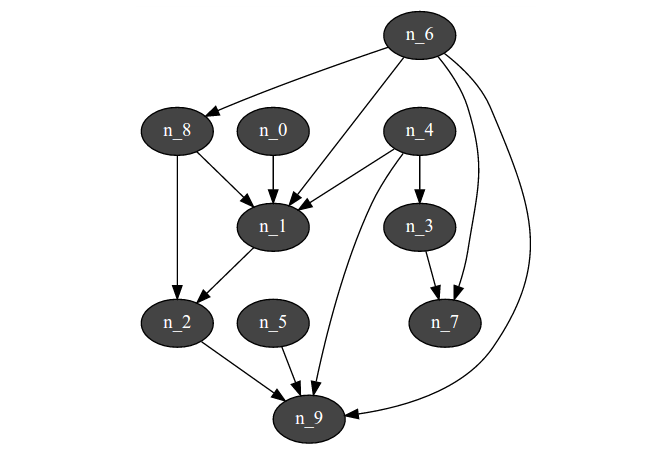
\includegraphics[width=\linewidth]{Images/Bayesian_Network.png}
  \label{fig:bng}  
 \end{subfigure}%
\begin{subfigure}{.5\textwidth}
  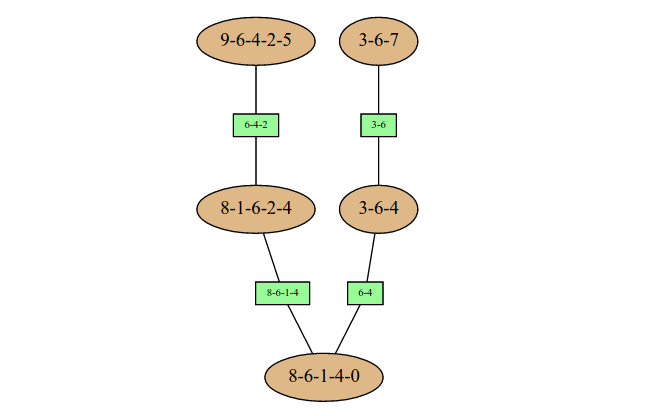
\includegraphics[width=\linewidth]{Images/Junction_Tree.png}
  \label{fig:jtg}  
 \end{subfigure}
 \caption{Un réseau bayésien généré (à gauche), et un arbre de jonction possible pour ce réseau (à droite)}
\end{figure}
\par \medbreak 
La première étape de création de ces arbres est une phase de 'moralisation' : il s'agit de créer un lien entre deux parents d'un même élémént. Dans l'exemple de la Figure 2, un lien est crée entre n2 et n5, 
deux des parents de n9. Une fois cette moralisation effectuée, la création de 'supercliques' regroupant des élèments connectés du réseau bayésien est quasiment finie. Toute orientation est ensuite enlevée, et la dernière
étape est une phase dite de 'triangulation', pour enlever toute possibilité de cycles à la nouvelle structure.

\end{document}